\documentclass[12pt,a4paper]{article}
\usepackage[utf8]{inputenc}
\usepackage{amsmath}
\usepackage{amsfonts}
\usepackage{amssymb}
\usepackage{graphicx}
\usepackage[margin=0.9in]{geometry}


\begin{document}
\title{Experimento 01 - Pêndulo Composto}
\author{Pedro Stringhini 
		\texttt{RA 156983}
		\and
		Lucas Schanner 
		\texttt{RA 156412}}
\maketitle
\newpage
\section{Resumo}

\section{Objetivos}
Investigar o movimento de um pêndulo e seu comportamento relacionando as grandezas sobre ele atuantes, como o centro de massa, o momento de inércia.

\section{Procedimento Experimental e Coleta de Dados}
\subsection{Procedimento}

Um pêndulo foi montado com uma barra metálica maior e outra adicional colocada em sua extremidade inferior. Ele, depois de devidamente medido (fita métrica) e pesado (balança), foi fixado em um eixo de suspensão. No ponto mais baixo da trajetória do instrumento, foi acoplado um photogate ligado à um cronômetro inteligente adaptado a medição dos periodos (T) de oscilação do pêndulo. Assim, com o devido cuidado de acionar uma oscilação de ângulo menor que 15 graus para efeitos de aproximação, foram medidos tais períodos 7 vezes em cada uma das 6 configurações escolhidas, diferenciadas quanto às distâncias entre eixo fixo e centro de massa do pêndulo.\\

\subsection{Dados Obtidos}

As medidas da posição do centro de massa das barras, relativo à extremidade inferior do pêndulo, são: \\
$ x_1 = (0.0915 \pm 0.0005) M$\\
$ x_2 = (0.7420 \pm 0.0005) M$\\


E suas Massas:\\
$ M_1 = (347.3 \pm 0.1) g $\\
$ M_2 = (929.5 \pm 0.1) g $\\


As medidas de periodo tomadas estão presentes na seguinte tabela, relacionadas as distâncias do eixo de rotação à extremidade inferior do pêndulo. \\

\begin{table}
\def\arraystretch{1.5}
\begin{tabular}{|l| c c c c c c c|r|}
\hline 
X (M) & \multicolumn{7}{c|}{Medidas de Periodo (s)} & Valor Médio \\ 
\hline
1.0450 & 1.8866 & 1.8878 & 1.8881 & 1.8869 & 1.8867 & 1.8862 & 1.8864 & $1.8870 \pm 0.0003 $ \\
\hline
0.9900 & 1.8877 & 1.8882 & 1.888 & 1.888 & 1.8851 & 1.8874 & 1.8869 & $1.8873 \pm 0.0004 $\\
\hline
0.9400 & 1.9018 & 1.9026 & 1.9020 & 1.9048 & 1.902 & 1.9016 & 1.8985 & $1.9019 \pm 0.0007$\\
\hline
0.8900 & 1.9341 & 1.9349 & 1.9345 & 1.9342 & 1.9335 & 1.9335 & 1.9340 & $1.9341 \pm 0.0002$\\
\hline
0.8400 & 1.9956 & 1.9957 & 1.9947 & 1.9947 & 1.9946 & 1.9986 & 1.9935 & $1.9953 \pm 0.0006$\\
\hline
0.7915 & 2.1042 & 2.1027 & 2.1027 & 2.1024 & 2.1026 & 2.1023 & 2.1019 & $2.1027 \pm 0.0003 $\\
\hline
 
\end{tabular} 
\caption{Medidas do Periodo de oscilação do pêndulo e suas médias aritméticas relacionadas à distância X do eixo de rotação à extremidade inferior do pêndulo. As medidas estão em Metros e Segundos. O erro no período foi calculado com base no erro estatístico e erro instrumental do cronômetro($0.0001 s$). O erro instrumental em X é $0.0005M$}
\end{table}




\section{Análise dos Resultados e Discussões}
\subsection{Centro de Massa}
A posição do do centro de Massa relativo a extrememidade inferior pode ser calculado como\\
$$ x_{cm} = \frac{x_1 \cdot M_1 + x_2 \cdot M_2}{M_1 + M_2} = 0.555 M $$\\ \\
O erro associado à essa medida, propagado a partir dos erros de $x_1$, $M_1$, $x_2$ e $M_2$ é de $$ \Delta x_{cm} =  0.009 M $$


\subsection{Períodos}
A equação $$ T = 2\pi\sqrt{\frac{D + \frac{k^2}{D}}{g}} $$ 
Pode ser reescrita como 
$$ T^2D = \frac{4\pi^2}{g} \cdot D^2 + \frac{4\pi^2}{g} \cdot k^2 $$ 
Então deve existir uma relação linear entre $T^2D$ e $D^2$


  
\begin{table}[!htbp]
\def\arraystretch{1.5}
\begin{tabular}{|c|c|c|c|}
\hline
D (M)& T(s) & $D^2$ & $T^2D$ \\
\hline
0.4897 & 1.8870 & 0.2399 & $1.74 \pm 0.03$\\
\hline
0.4347 & 1.8873 & 0.1890 & $1.55 \pm 0.03$\\
\hline
0.3847 & 1.9019 & 0.1480 & $1.39 \pm 0.03$\\
\hline
0.3347 & 1.9341 & 0.1121 & $1.25 \pm 0.03$\\
\hline
0.2847 & 1.9953 & 0.0811 & $1.13 \pm 0.04$\\
\hline
0.2362 & 2.1027 & 0.0558 & $1.04 \pm 0.04$\\
\hline
\end{tabular} 


\caption{Periodos de oscilação relacionados à distância $D$ dos eixo de rotação ao centro de massa. O erro em D é constante igual a $0.009 M$ (propagado a partir do erro em X e em $x_{cm}$) e o erro em $T^2D$ foi propagado a partir do erro em D e em T.}
\end{table}

Fazendo a regressão linear de $T^2D$ X $D^2$ por mínimos quadrados, obtemos os coeficientes $$ a = 3.8 \pm 0.2 $$ e $$ b = 0.83 \pm 0.04 $$ onde $a$ é o coeficiente angular e $b$ é o coeficiente linear.

\begin{figure}[h]
\caption{Gráfico de $T^2D$ em função de $D^2$. Nota-se que os dados coletados se encaixam muito bem em uma projeção linear.}
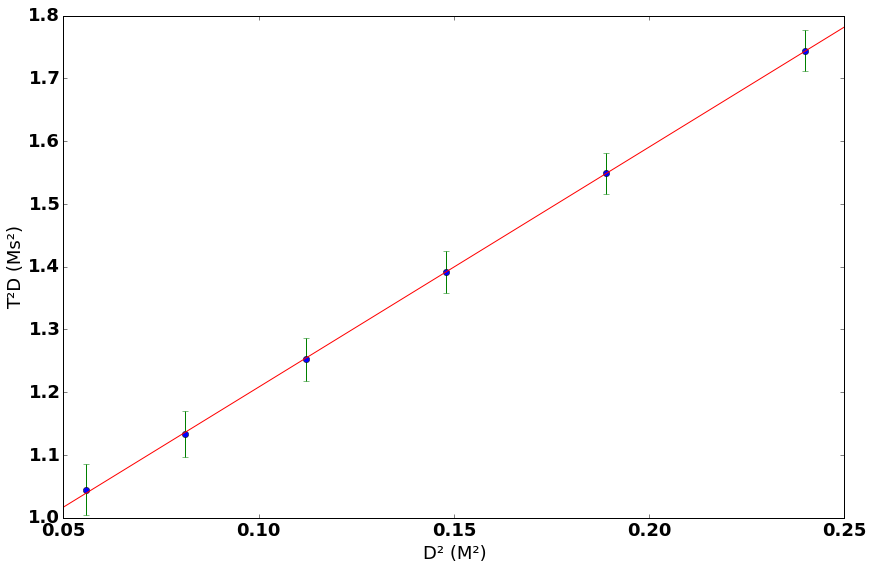
\includegraphics[scale=0.55]{index.png} 

\end{figure}
\subsection{Gravidade}
A interpretação física do coeficiente angular encontrado é $$ a = \frac{4\pi^2}{g} = 3.8 \pm 0.2$$ logo podemos encontrar g como $$ g = \frac{4\pi^2}{3.8} = 10.32$$ e seu erro associado, propagado a partir do erro em $a$ é $ \pm 0.05 $
\subsection{Raio de giração}
\subsection{Momento de Inércia}




\section{Conclusões}

\end{document}